\documentclass[11pt]{article}
\usepackage[utf8]{inputenc}
\pagestyle{headings}
\usepackage[top=1in, bottom=1in]{geometry}
\usepackage{amsmath,amsfonts,amsthm,amssymb}
\usepackage[pdftex]{graphicx}
\usepackage{url}
\usepackage{subfig}
\usepackage{color}
\usepackage[pagebackref=true,breaklinks=true,letterpaper=true,colorlinks,bookmarks=false,citecolor=red,linkcolor=blue]{hyperref}

%% Command definitions
\def\subsectionautorefname{section}
\newcommand{\note}[1]{\textcolor{red}{\textbf{#1}}}
\definecolor{light-gray}{gray}{0.3}
\newcommand{\aside}[1]{\textcolor{light-gray}{\emph{#1}}}
\newcommand{\comment}[1]{}

\title{Attentional Object Detection: A Proposal}
\author{Sergey Karayev}
\date{updated: 22 April 2011}

\begin{document}
\maketitle

\begin{abstract}
This document tracks the development of ideas for efficient object detection using the idea of attention: a sequential process of looking for something somewhere.
We follow the Deformable Part Model approach to object detection and extend it in several ways, mostly focusing on the role of context, toward the goal of Anytime detection performance.
I expect a submission to NIPS'11 to be whittled down from the text and results here.
\end{abstract}

\tableofcontents
\newpage

%!TEX root=paper/paper.tex
\chapter{Introduction}\label{sec:introduction}

\section{Motivation}

\PM{Perception}
It is well-known that human perception is Anytime, meaning that a scene can be described after even a short presentation.
Perception is also progressive, meaning that the quality of description increases with more time.
The progressive time course of visual perception has been confirmed by multiple studies \parencite{Vanrullen-1996,Fei-Fei-Vision-2007}, with some studies providing evidence that enhancement occurs in an ontologically meaningful way.
For example, people tend to recognize something as an animal before recognizing it as a dog \parencite{Mace-PloS-2009}.
The underlying mechanisms of this behavior are unknown, and only a few attempts have been made to explain the temporal dynamics (for instance, a promising work by \cite{Hegde-Neuro-2008} has employed the framework of sequential decision processes).

\PM{Computer applications}
Meanwhile, automated visual recognition has achieved levels of performance that allow useful real-world implementation.
We focus on two problem formulations: \emph{image classification}, in which some property of the image -- such as scene type, visual style, or even object presence -- is predicted, and \emph{object detection}, in which the location and category (or identity) of all objects in a scene is predicted.
Solutions to the two problems are often linked, as classification can be a subroutine for detection.
Our motivation is that state-of-the-art methods for classification and detection tend to be computationally expensive, insensitive to Anytime demands, and not progressively enhanced.

\PM{Application}
As real-world deployment of recognition methods grows, managing resource cost (power or compute time) becomes increasingly important.
For tasks such as personal robotics, it is crucial to be able to deploy varying levels of processing to different stimuli, depending on computational demands on the robot.
A hypothetical system for vision-based advertising, in which paying customers engage with the system to have their products detected in images on the internet, presents another example.
The system has different values (in terms of cost per click) and accuracies for different classes of objects, and the backlog of unprocessed images fluctuates based on demand and available server time.
The recognition strategy to maximize profit in such an environment should exploit all signals available to it, and the quality of detections should be Anytime, depending on the length of the queue (for example, lowering recall when queue pressure grows).

\PM{Visual Features / Classification}
For most state-of-the-art classification methods, a range of features are extracted from an image instance and used to train a classifier.
Since the feature vectors are usually very high-dimensional, linear classification methods are used most often -- for instance, logistic regression.
Features are extracted at different costs, and contribute differently to decreasing classification error.
Although it can generally be said that ``the more features, the better,'' high accuracy can of course be achieved with only a small subset of features for some instances.
Additionally, different instances benefit from different subsets of features.
For example, simple binary features are sufficient to quickly detect faces \parencite{Viola-IJCV-2004} but not more varied visual objects, while the features most useful for separating landscapes from indoor scenes \parencite{Xiao-CVPR-2010} are different from those most useful for recognizing fine distinctions between bird species \parencite{Farrell-ICCV-2011}.
\autoref{fig:features} presents several common visual features.

\PM{Detection}
Detection methods tend to employ the same visual features and classifiers but apply them to many image sub-regions.
Approaches can broadly be grouped into \emph{per-class, exhaustive-region}, \emph{all-class, exhaustive-region}, and \emph{all-class, proposed-region} methods.
State-of-the-art \emph{per-class, exhaustive-region} methods such as \cite{Felzenszwalb2010a} and \emph{all-class, proposed-region} methods such as \cite{Girshick-CVPR-2014} are considerably slow, performing an expensive computation on a thousand to a million image windows.
To maximize early performance gains of these methods, scene and inter-object contextual cues can be exploited in two ways.
First, regions can be processed in an intelligent order, with most likely locations selected first.
Second, if detectors are applied per class, then they can be sequenced so as to maximize the chance of finding objects actually present in the image.
And even the most recent \emph{all-class, exhaustive-region}, Convolutional Neural Net (CNN)-based detection methods such as \cite{He-ECCV-2014}, which take advantage of high-performance convolutional primitives for region processing and detect for all classes simultaneously, can be sped up using Anytime ideas such as cascaded classification.

\section{Our Work}

\PM{Costliness}
Computing all features, running all detectors, or processing all regions for all images is infeasible in a deployment sensitive to Anytime needs, as each feature brings a significant computational burden.
Yet the conventional approach to evaluating visual recognition does not consider efficiency, and evaluates performance independently across classes.
We address the problem of selecting and combining a subset of features under an Anytime cost budget, specified in terms of wall time or total power expended or another metric, and propose a new \emph{costliness} measure of performance vs. cost.

\PM{Learning a Policy}
To exploit the fact that different instances benefit from different subsets of features, our approach to feature selection is a sequential policy.
To learn the policy parameters, we formulate the problem as a Markov Decision Process (MDP) and use reinforcement learning methods.
The method does not make many assumptions about the underlying actions, which can be existing object detectors and feature-specific classifiers.
With different settings of parameters, we can learn policies ranging from \textbf{Static, Myopic}---greedy selection not relying on any observed feature values, to \textbf{Dynamic, Non-myopic}---relying on observed values and considering future actions.
The foundational machinery is laid out in \autoref{sec:det_method}.

\PM{Per-class Detection}
For \emph{per-class} detection, the actions are time-consuming detectors applied to the whole image, as well as a quick scene classifier.
We run scene context and object class detectors over the whole image sequentially, using the results of detection obtained so far to select the next actions.
Since the actions are time-consuming, we use a powerful inference mechanism to select the best next action.
In \autoref{sec:det_evaluation}, we evaluate on the PASCAL VOC dataset and obtain better performance than all baselines when there is less time available than is needed to exhaustively run all detectors.

\PM{Image Classification}
Classification actions are much faster than detectors, and the action-selection method accordingly needs to be fast.
Because different features can be selected for different instances, and because our system may be called upon to give an answer at any point during its execution, the feature combination method needs to be robust to a large number of different observed-feature subsets.
In \autoref{sec:clf_chapter}, we consider several value-imputation methods and present a method for learning several classifiers for different clusters of observed-feature subsets.
We first demonstrate on synthetic data that our algorithm learns to pick features most useful for the specific test instance.
We demonstrate the advantage of non-myopic over greedy, and of dynamic over static on this and the Scene-15 visual classification dataset.
Then we show results on a subset of the hierarchical ImageNet dataset, where we additionally learn to provide the most specific answers for any desired cost budget and accuracy level.

\PM{Cascaded CNN}
We additionally investigate a novel approach for speeding up a state-of-the-art CNN-based detection method, and propose a general technique for accelerating CNNs applied to class imbalanced data.
We bring the classic idea of the cascade to CNNs by inserting a \emph{reject} option between CNN layers.
When the CNN processes batches of images, which is standard for many applications, the reject layers allows the CNN to ``thin'' the batch as it progresses through the network, thus saving processing time.
This method is applicable to both \emph{all-class, proposed-region} methods such as \cite{Girshick-CVPR-2014} and \emph{all-class, exhaustive-region} methods such as \cite{He-ECCV-2014}.
We demonstrate results --- along with a variety of strong baselines -- on the former method, and show that the Cascaded CNN method obtains a nearly 10x speed-up with only marginal drop in accuracy.
All work is reported in \autoref{sec:ccnn_chapter}.

\PM{Recognizing Style}
Lastly, in \autoref{sec:style_chapter}, we present two novel datasets and first results for an underexplored research problem in computer vision -- recognizing visual style.
In preparation for an Anytime approach, we evaluate several different features (including CNNs) for the task, and explore content-style correlations in our datasets.
Our large-scale learning gives state-of-the-art results on an existing dataset of image quality and photographic style, and provides a strong baseline on our contributed datasets of 80K photos and 85K paintings labeled with their style and genre.
In a demonstration of cross-dataset understanding of style, we show how results of a search by content can be filtered by style.

\PM{Future Directions}
This works provides an effective foundation for further exploration of Anytime recognition, and points the way to interesting further development.
Our MDP-based formulation of learning a feature-selection policy is empirically effective, but heuristic in nature.
The recently developed framework of adaptive submodularity \parencite{Golovin-and-Krause-2010-JAIR} could provide theoretical near-optimality results for some policies, but developing an appropriate objective for our task is not straightforward.
We showed our Cascaded CNN model to be effective for a region-based detection task -- but the model was not trained end-to-end with the threshold layers.
An even more interesting future development would add an Anyitme loss layer that combines classification output from multiple levels of the network in a cost-sensitive way.
We explain these ideas in detail in \autoref{sec:conclusion}.

%!TEX root=paper/thesis.tex

%!TEX root=../paper/paper.tex
\section{Evaluation}\label{sec:ccnn_evaluation}

\PM{Dataset}
We evaluate on the standard object detection benchmark: the PASCAL VOC \cite{pascal-voc-2010}.
In all cases, the CNN region classifiers are trained on the PASCAL VOC 2007 trainval set.
The parameters of our methods are set by training or cross-validation on the VOC 2007 val set.
We evaluate on the VOC 2007 test set.
The result plots and details are shown in \autoref{fig:voc2007_results} and \autoref{tab:ccnn_results}.

\PM{Implementation}
The scoring function for the quick-to-compute features is trained by a logistic regression classifier onto the max PASCAL overlap with any ground truth window on the validation dataset.
The classifier is optimized by stochastic gradient descent, and its regularization parameter is cross-validated.
The R-CNN software was used as available in June 2014.
\footnote{\url{https://github.com/rbgirshick/rcnn}}
That software relies on Selective Search \cite{Uijlings-IJCV-2013} region proposals.
Different images are proposed different numbers of regions.
\autoref{fig:roi_hist} shows the distribution of number of regions on the validation set, with the parameters of the R-CNN.
An additional parameter is the size of each batch of regions that goes through the CNN.
We set batch size to 100 regions, and observe that it takes on average 500 ms to process them with the CNN.
In all experiments, we use Ubuntu 12.04, Intel i5 3.2GHz CPU, and NVIDIA Tesla K40 GPU.

%!TEX root=../paper/paper.tex
\begin{figure}[ht]
\begin{subfigure}[b]{\linewidth}
    \centering
    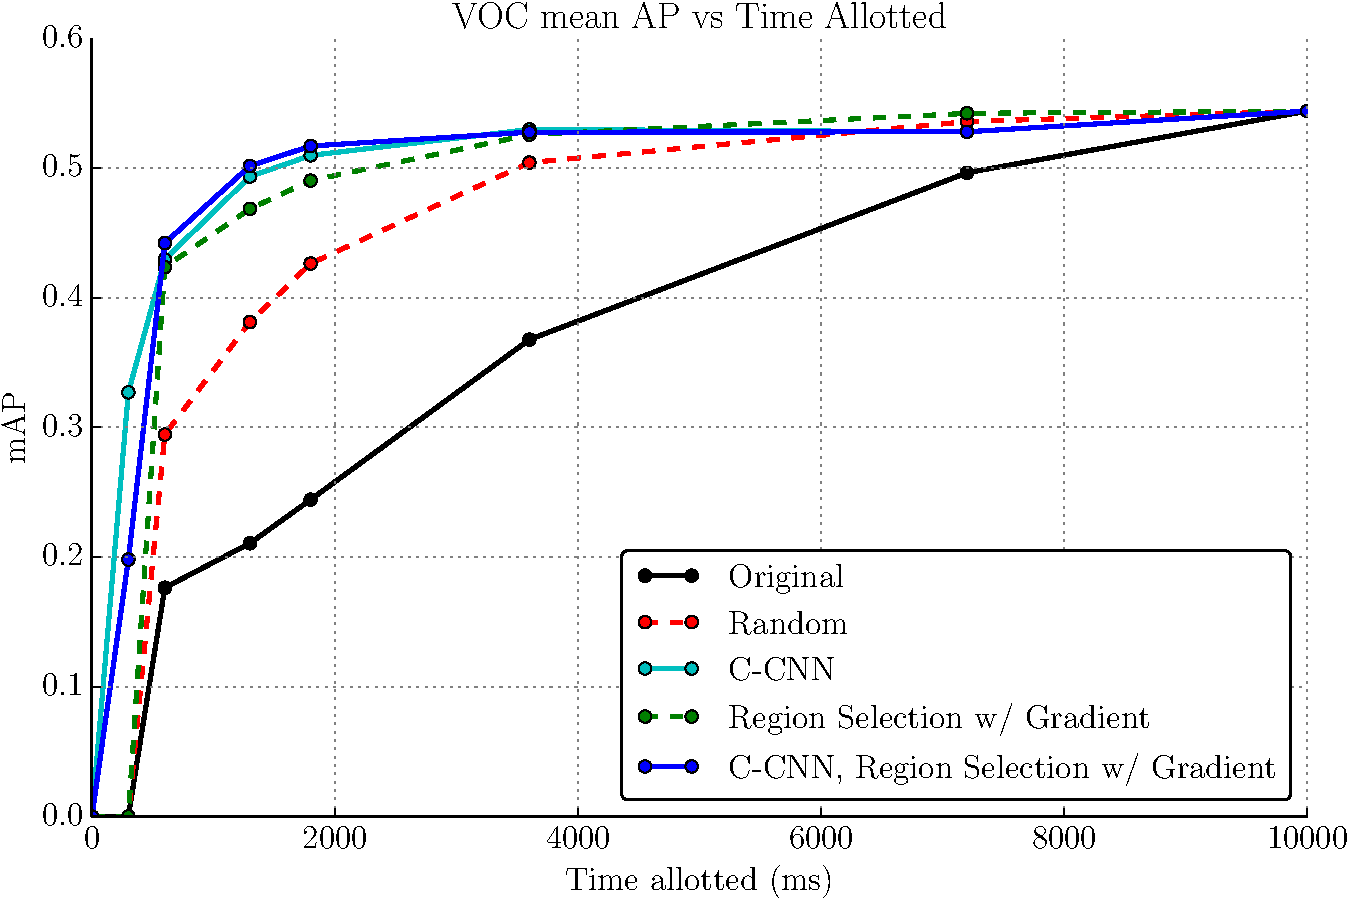
\includegraphics[width=.75\linewidth]{../ccnn/figures/_apvst_final.pdf}
    \caption{
Plotting Mean AP vs. Time Allotted allows comparison performance at a given time budget.
For example, at 1300 ms, random region selection gets about 0.42 mAP, while our best method (C-CNN with gradient-based region selection) obtains 0.50 mAP.
}\label{fig:apvst}
\end{subfigure}
\begin{subfigure}[b]{\linewidth}
    \centering
    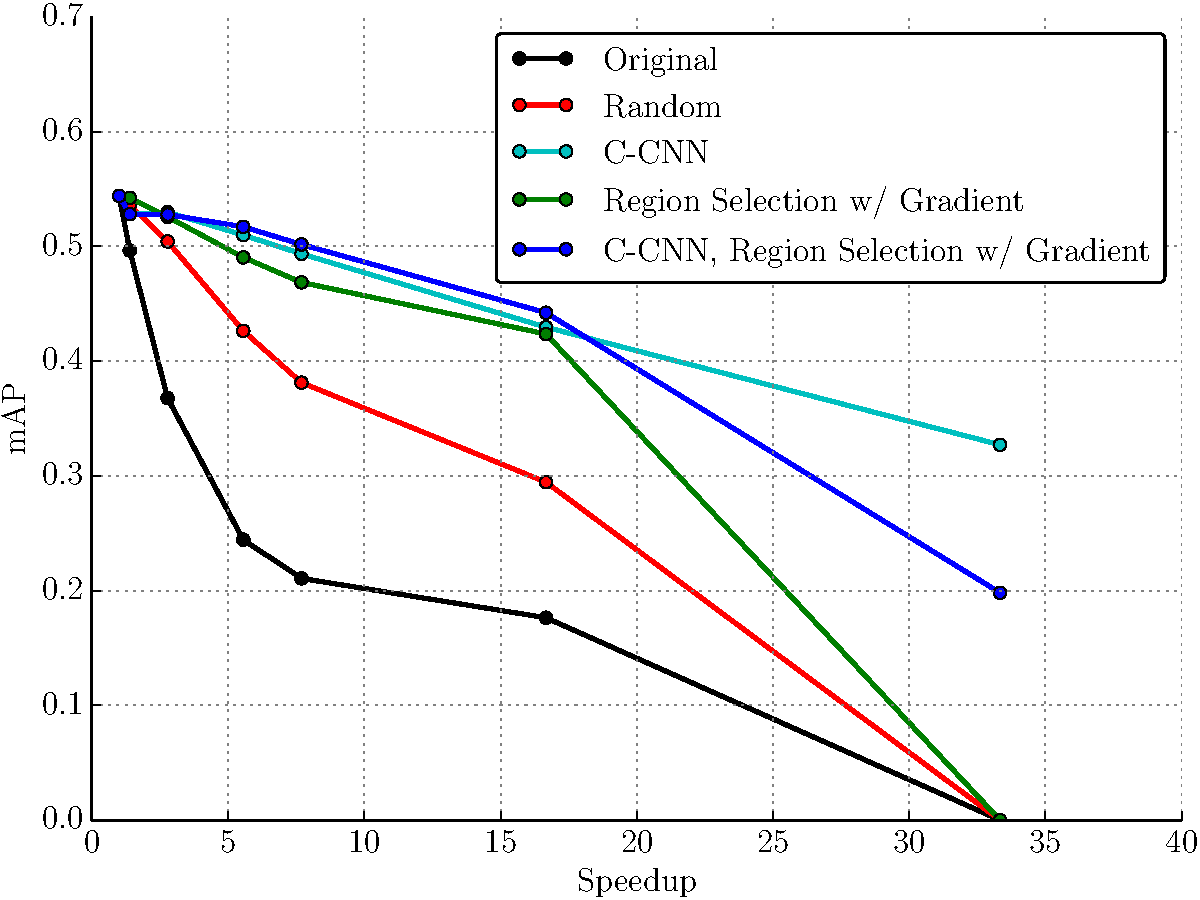
\includegraphics[width=.75\linewidth]{../ccnn/figures/_speedup_final_abs.pdf}
    \caption{
Plotting mean AP vs. speed-up factor allows comparison of speed-ups at a given mAP point.
For example, we can see that we should obtain mAP of 0.40 at around 20x speedup with our method.
}\label{fig:speedup}
\end{subfigure}
\caption{
Results of the Cascade CNN and other Anytime methods on the PASCAL VOC 2007 dataset.
}\label{fig:voc2007_results}
\end{figure}


\begin{table}[ht]
\centering
\caption{
Full table of AP vs. Time results on PASCAL VOC 2007.
Best performance for each time point is in bold.
}\label{tab:results}
\small{
\begin{tabular}{lrrrrrrrr}
\toprule
Time allotted (ms)                  & 0 & 300            & 600            & 1300           & 1800           & 3600           & 7200           & 10000 \\
\midrule
Original                            & 0 & 0.000          & 0.176          & 0.211          & 0.244          & 0.368          & 0.496          & 0.544 \\
Random                              & 0 & 0.000          & 0.295          & 0.381          & 0.426          & 0.504          & 0.536          & 0.544 \\
C-CNN                               & 0 & \textbf{0.327} & 0.430          & 0.493          & 0.510          & 0.528          & 0.528          & - \\
Region Selection w/ Gradient        & 0 & 0.000          & 0.424          & 0.469          & 0.490          & 0.526          & \textbf{0.542} & 0.544 \\
C-CNN, Region Selection w/ Gradient & 0 & 0.198          & \textbf{0.442} & \textbf{0.502} & \textbf{0.517} & \textbf{0.528} & 0.528          & - \\
\bottomrule
\end{tabular}
}
\end{table}


The experimental settings are
\begin{description}
  \item[Original] \hfill \\
  The original order of the Selective Search regions of interest.
  This order is influenced by the hierarchical segmentation of their method, and so has sequences of highly overlapping regions.

  \item[Random] \hfill \\
  A completely blind permutation of the original order.

  \item[Region Selection] \hfill \\
  The region statistics feature is always used.
  Additionally, we consider the Pixel Gradient feature, with \emph{setup time} of the gradient forward-back propagation of 20 ms.

  \item[Cascaded CNN] \hfill \\
  The Cascaded CNN model, as described in \autoref{sec:ccnn}.
  The first experiment (C-CNN) takes batches of regions in a random order.
  The next two experiments also make use of the Region Selection methodology with the quick-to-compute feature.
\end{description}

\PM{Analysis}
Since the time to process a full batch with a non-cascaded CNN is 500 ms, there are no results for non-cascaded baselines at 300 ms.
At this time, the Cascaded CNN without any region ordering is best.
A reason for why C-CNN with Region Selection is not as good at this point is that the region selection presents better region candidates, with fewer rejection opportunities, and thus has less coverage of the image.
At 600 ms, C-CNN method have had more than one batch go through, and the Region Selection is giving it a lead over the simple C-CNN.
Both method are better than the baseline non-cascaded methods for this entire duration.

\section{Our Approach}

\subsection{Assumptions and Notations}
\begin{table}
\centering
  \caption{Summary of our notation.}
  \begin{tabularx}{0.85\textwidth}
  {| l | X |}
  \hline
  Term &      Definition \\
  \hline
  $D$ &     Set of images $d$ composing the dataset. \\
  $K$ &     Set of object classes $k$ present in the dataset. \\
  $C$ &     Set of classifiers $c_{k,i}$, where $k \in K$ and $1 \leq i \leq |C_k|$ allows the possibility of more than one classifier per class. \\
  $|C_k|$ & Number of classifiers for class $k$. \\
  \hline
  \end{tabularx}
\label{tab:notation}
\end{table}

We have a dataset of images $d \in D$.
Each image contains at least one object with class $k \in K$.
``Background'' is not considered to be a class.

For each class $k$, we have $|C_k|$ classifiers $c_{k,i}$, with $1 \leq i \leq |C_k|$.
$|C_k|$ must be at least $1$, but there may be more than one classifier per class---for example, a slow but powerful and a fast but weak classifier for each class.

The task of object detection is defined as evaluating windows (bounding boxes) in the image with these classifiers.
This is a common formulation; if the window proposals are exhaustive and the classifiers are perfect, then all objects in the image should be perfectly localized.
An important aside is the role of post-processing of detections.
Because a single ground truth bounding box will give rise to multiple correct detections (the overlap requirement is not 1), but only one detection can be counted as correct for a given bounding box according to the PASCAL evaluation, detections are usually reduced with non-maximum suppression, which finds the bounding box with the highest confidence.
The score of a classifier should then correspond to the amount of overlap with the ground truth, not only to the binary presence decision.

Following~\cite{Lehmann2011}, we parameterize a window $w$ by its center $(x,y)$, scale $s$, and aspect ratio $r$.
While some classifiers are able to handle a window of any dimensions, some expect to evaluate windows of a certain aspect ratio, and may be sensitive to the scale.
Accordingly, the bounds on $s$ and $r$ depend on the model of the classifier.
The set of possible window proposals for an image of size $n \times m$, according to the model of classifier $c_{k,i}$ is therefore defined by $W_{k,i} = \left\{ x,y,s,r | x \in [0,m], y \in [0,n], s \in [\underline{s}_{k,i}, \overline{s}_{k,i}], r \in [\underline{r}_{k,i}, \overline{r}_{k,i}] \right\}$.

This notation is also summarized in Table~\ref{tab:notation}.

In a nutshell, our approach consists of
\begin{itemize}
\item Modeling the classifier toward the goal of inferring the object posterior from classifier scores.
\item Maintaining prior distributions over the object class presence in a region.
\item Updating the priors for all classes after inferring the posterior of one class by running a detector.
\end{itemize}

\subsection{Modeling the Classifier}
A classifier $C_k$ takes an image window $w$ and answers the question, ``is the object of class $k$ present in window $w$?''
For shorthand, we define $w_K$ to be the class of object present in window $w$.

We model $C_k$ with two distributions over its confidence: $P(score | w_K = k)$ and $P(score | w_K \neq k)$.
We model the score likelihood distributions with, for example, the Beta distribution, and learn the parameters from data.

The score (confidence) of the classifier is supposed to represent the posterior $P(w_K = k | \Psi(w), C_k)$, where $\Psi(w)$ represents the features extracted from $w$, according to the model of $C_k$.
But of course, the score is affected by lossy signal and limited by the modeling capacity of $C_k$.
A classifier that is not able to model the object class or is overrun by noise will have a uniform distribution.
A perfect classifier will have two point distributions at the $1$ and $0$ values.

To infer the $P(w_K=k)$ from the classifier score, we can write:
\[
P(w_K=k|score) = \frac{P(score|w_K=k)P(w_K=k)}{P(score|w_K=k)P(w_K=k)+P(score|w_K \neq k)P(w_K \neq k)}
\]

In this way, the score of a worthless classifier will not play a role in determining the object posterior, and the score of a perfect classifier will completely override the role of the prior.

\subsection{Detectors, not Classifiers}
Up until now, we have ignored the fact that our classifiers are run not just on a single window but on a set of windows in the image region.
Accordingly, we obtain a \emph{list} of detections instead of a single score after running $C_k$ in an image region.

Our class priors are defined as the probability of an object of the given class being present in any given window in the image region.
Therefore, the priors are sensitive to the size of the region relative to the size of the image, and to the resolution of the image.

\note{there is something here about the gradient from classification to detection, but i'm not sure what it is... need to think more}

\subsection{Window Discretization}
We follow \cite{Zhang2011} in our window discretization scheme, which we summarize here.
We define the overlap between window $t \in T$, the set of all possible windows in the image, and window $s \in S$, the set of all windows with width $w$ and height $h$ according to the PASCAL overlap criterion:
\begin{equation}
o(t,s) = \frac{t \bigcap s}{t \bigcup s}
\end{equation}

We say that $s$ is represented to $\eta$-accuracy if $o(t,s) \leq \eta$. 

\subsection{Object Co-Occurrence}
The object posterior that we inferred from running the detector is information that we should take into account when picking the next action.
We can certainly replace the current prior for this class with the posterior, but we also want to influence the priors on the other classes.

We model the object class cooccurrence with a fully connected field of $K$ random variables $P(w_K=k)$, one per class.
The variables 




\section{Location Discretization and Feature Computation} \label{sec:discretization_and_featurization}

\paragraph{Location Discretization}
The fewer possible discrete locations $l_i = (x,y,s)$, with $i = 1 \dots N$, we consider, the smaller our state space and therefore the better our reinforcement learning solution for a given amount of computation.
Featurization also takes less time as tolerable coarseness increases.
At the same time, we lose power to match ground truth detections.

There are three factors in the discretization process: the stride of the center point of the window $(x,y)$, and the number of octaves and scales per octave of $s$.

\note{todo: include a figure plotting oracle performance vs. decreasing coarseness of the image pyramid discretization.}

\paragraph{Coarse-to-Fine Evaluation}
The standard scale-invariant approach to detection with a template is to evaluate a template of fixed size over different scales of the image pyramid.
A recent report makes the observation that this approach using high-resolution, part-based models performs worse than scale-variant detection that degrades to using low-resolution, rigid models for detection at small scales of the image~\cite{Park2010}.
They demonstrate state-of-the-art results on a pedestrian detection benchmark.
The authors also note that context is most helpful for small-object detections.

\begin{figure}[h!]
  \caption{Illustration of the idea of using low-res models to approximate the output of high-res models, allowing us to only compute the image pyramid at small scales.}
  \centering
    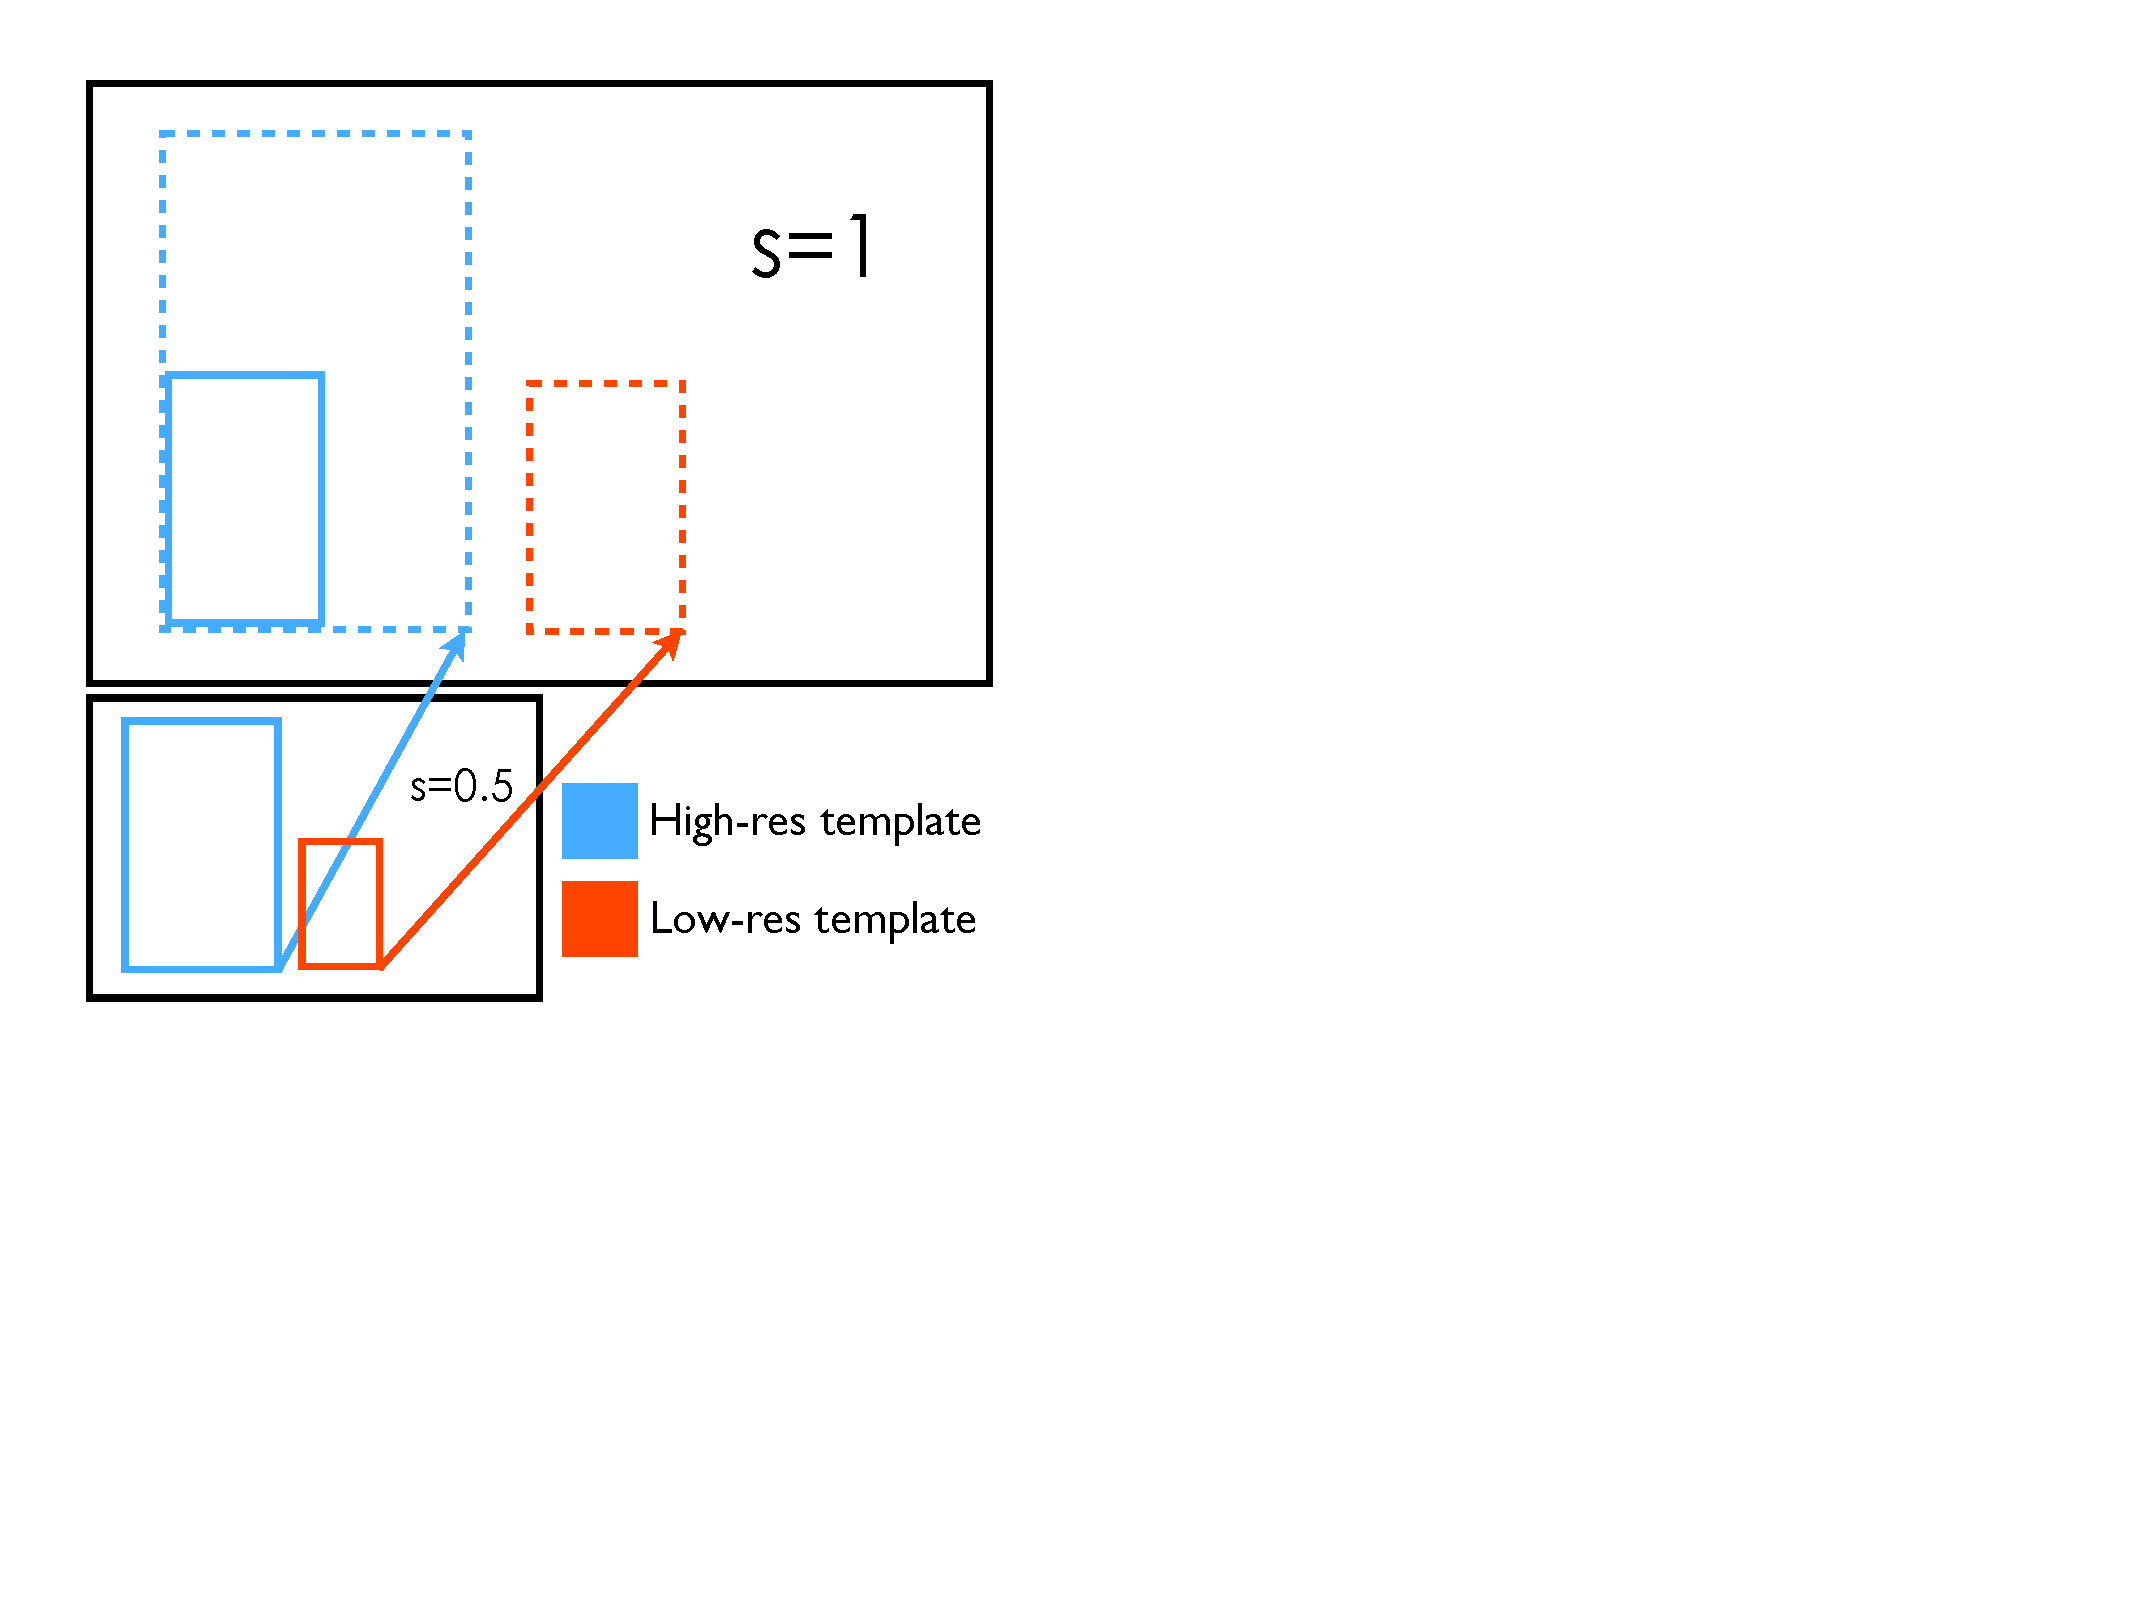
\includegraphics[width=0.7\textwidth]{../figures/multiscale.pdf}
  \label{fig:multiscale}
\end{figure}
We note also that a low-resolution model used at scale $s/2$ provides an approximation to the output of a high-resolution model at scale $s$, as illustrated in~\autoref{fig:multiscale}.
This may allow us to stagger feature computation, first computing just the small-scale part of the pyramid and running low-res models, and then computing the the large-scale part of the pyramid as time allows.

\paragraph{Feature Computation}
\note{todo: how can we include feature computation as part of the action space?}

\note{should look at Piotr Dollar's work on efficient HOG computation~\cite{Dollar2010}.}
\section{Loose Ideas}

\subsection{Local context feature}
We could try augmenting the DPM model with a local context window, for example by learning another HOG template on a window that is slightly larger than the object window.
Has this been done, and why not?
It's also what Allie is thinking of doing for shadow (shadow context around object windows).

\subsection{Fast multi-class approximation of the right class} \label{sec:multiclass_approx}
If we consider a window and have $N$ detectors, how can we efficiently figure out which of the $N$ detectors have the greatest likelihood of giving a high score to this window?

One idea is to use classifier dimensionality reduction.
Let's assume we are using SVM classifiers and classifying vectors of the same dimension.
Do we really need to run all of them in their full dimensions, to have a good guess as to which are going to score high?
Could we not use dimensionality reduction on all the learned classifiers to come up with a very low-dimensional evaluation that would approximate the full-dimensional score?
Then we could only run those classifiers that are past threshold on this low-dimensional approximation.

Another idea is to forget about the specific classifier we are using and just try to partition the feature space into class clusters, roughly.
We can use K-means, for example.
The cluster(s) that a specific window then falls into determine the more complex classifiers that we will evaluate.

\aside{
A similar idea is explored in the paper \cite{Isukapalli2006}.
They use boosting to train a cascade of classifiers to classify all object classes.
Then they learn a policy to partition the output of the detectors into class-specific clusters.
The policy is a decision tree.
The leafs of the decision trees specify the expected class of that window, and they use that to run a class-specific classifier cascade.
}
\section{Results}

We want to show two things: 1) given the same amount of time as our baseline systems, we perform at least as well as them; 2) in the AP vs. time evaluation, we do better than all baselines.

\begin{description}
  \item[Cascaded DPM Baseline~\cite{Felzenszwalb2010b}] We should do as well as it does in the same time ($\approx$0.5 sec), and better than it for shorter times than that.
  \item[Coarse-to-fine Baseline~\cite{Pedersoli2011}] Same thing.
\end{description}

We should think of ways to make the comparison fair.

Should we run the multi-class NMS~\cite{Desai2009} over the detections of the baselines?
Since our approach relies on it, it seems that we should; on the other hand, it's part of the special sauce of our approach.

To make sliding window detectors run faster, we can modify the stride or scale quantization of their sliding window.
So, if we want to output detections in 0.1 seconds, we can modify the Cascaded DPM code, for example, to cover the image in that long.

\bibliographystyle{ieeetr}
\small
\bibliography{sergeyk-bibtex}
\end{document}
